\section{Markov Model}
\label{sec:MarkovModel}

This model is designed to import a generic Markov chain as a RAVEN model.
As an example, the Markov chain of Fig.~\ref{fig:markov} is translated in the OpenPSA as shown below:

\begin{figure}
    \centering
    \centerline{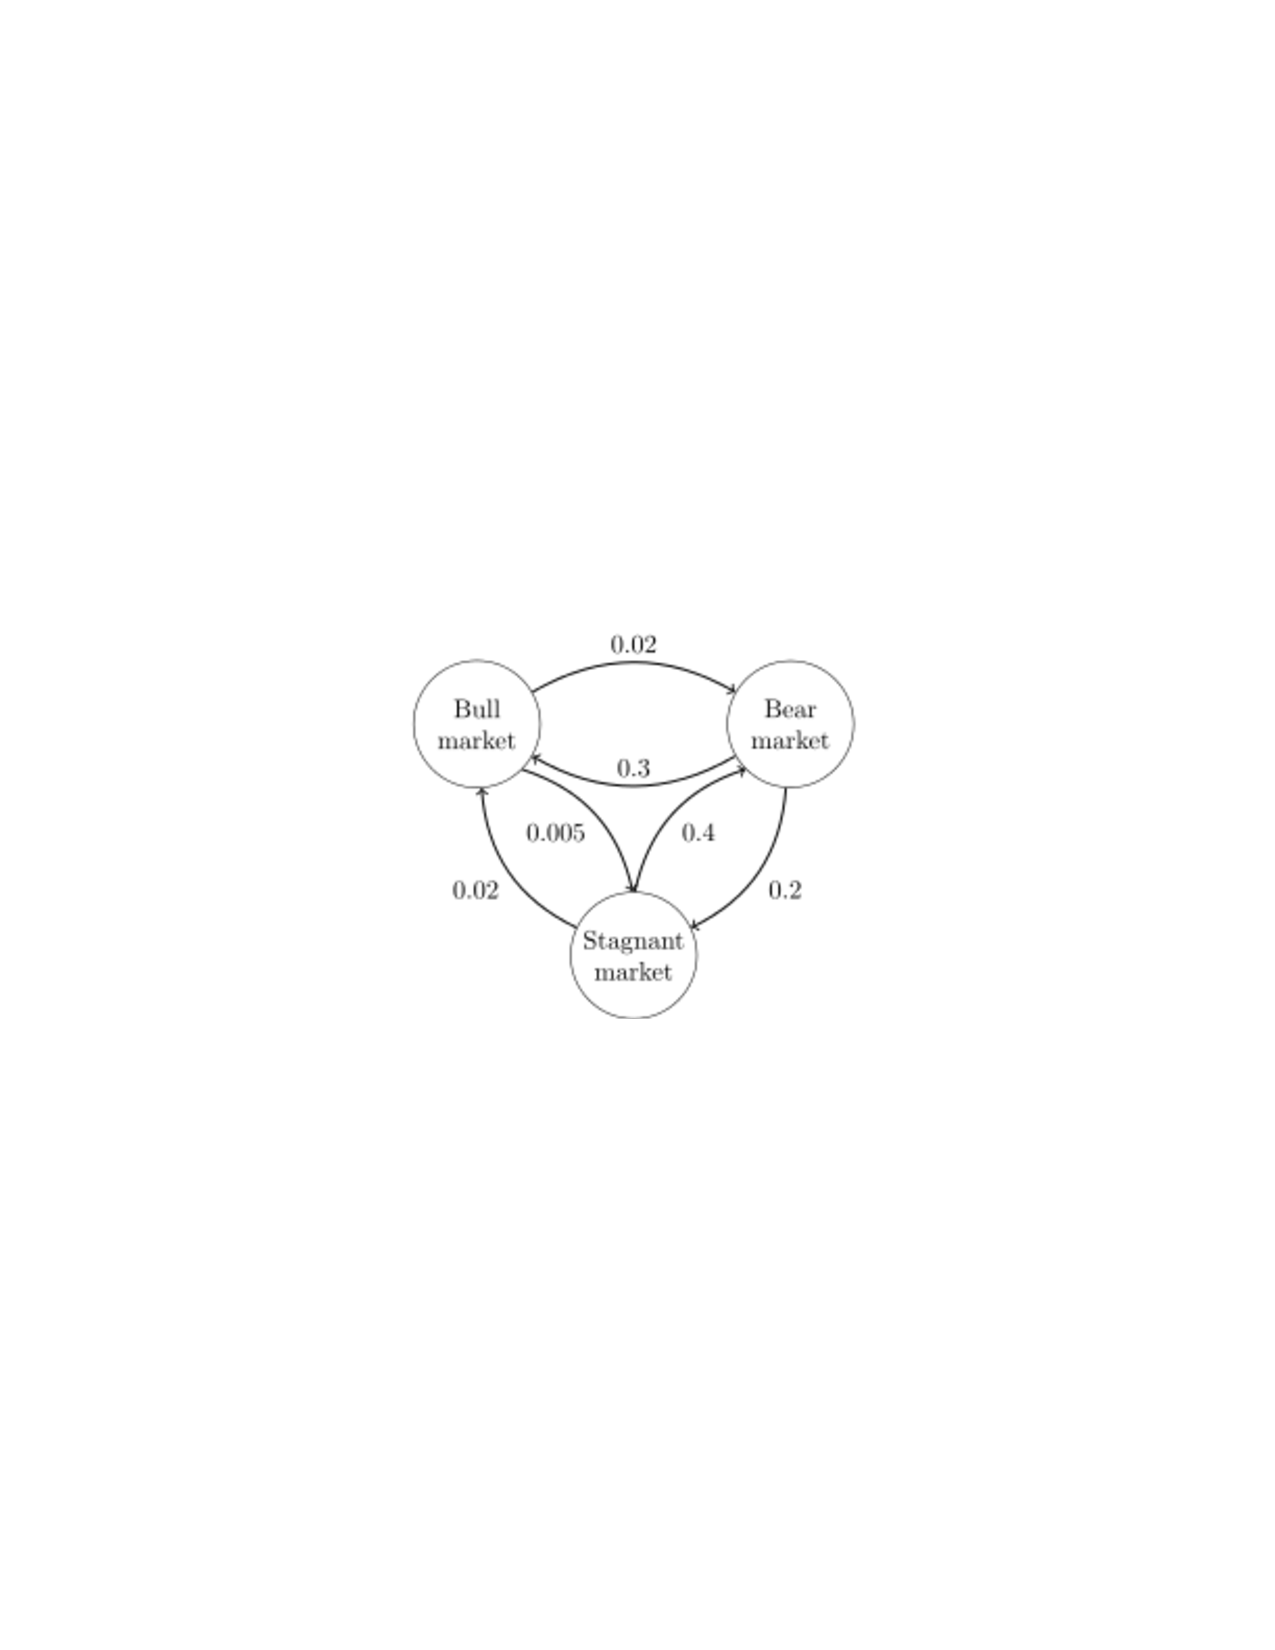
\includegraphics[scale=0.5]{markov.pdf}}
    \caption{Example of continuous time Markov chain (source Wikipedia: https://en.wikipedia.org/wiki/Markov\_chain).}
    \label{fig:markov}
\end{figure}

\begin{lstlisting}[style=XML,morekeywords={anAttribute},caption=Markov model input example., label=lst:Markov_InputExample]
  <Models>
    <ExternalModel name="markov" subType="MarkovModel">
      <variables>initialState,finalState</variables>
      <initState>initialState</initState>
      <finState>finalState</finState>
      <endTime>1000</endTime>
      <state name="1"> <!-- Bull market -->
        <transition type="lambda" value="0.02" >2</transition>
        <transition type="lambda" value="0.005">3</transition>
      </state>
      <state name="2"> <!-- Bear market -->
        <transition type="lambda" value="0.3">1</transition>
        <transition type="lambda" value="0.2">3</transition>
      </state>
      <state name="3"> <!-- Stagnant market -->
        <transition type="lambda" value="0.02">1</transition>
        <transition type="lambda" value="0.4" >2</transition>
      </state>
    </ExternalModel>
  </Models>
\end{lstlisting}

All the specifications of the Markov model are given in the \xmlNode{ExternalModel} block.
Inside the \xmlNode{ExternalModel} block, the XML nodes that belong to this model are:
\begin{itemize}
  \item  \xmlNode{variables}, \xmlDesc{string, required parameter}, a list containing the names of both the input and output variables of the model
  \item  \xmlNode{initState}, \xmlDesc{string, required parameter}, variable ID corresponding to initial state
  \item  \xmlNode{finState}, \xmlDesc{string, required parameter}, variable ID corresponding to final state
  \item  \xmlNode{endTime}, \xmlDesc{float, required parameter}, time horizon to evaluate Markov chain transition history
  \item  \xmlNode{state}, specifies a single node; inside a \xmlNode{state} all possible transitions OUT of this state must be specified
                          in the \xmlNode{transition} xml sub-nodes:
	  \begin{itemize}
	  	\item \xmlAttr{transition}, \xmlDesc{required string attribute}, arrival state
	    \item \xmlAttr{type}, \xmlDesc{required string attribute}, type of transition. Allowed transition types are:
      lambda, tau, instant and unif (see below)
	    \item \xmlAttr{value}, \xmlDesc{required string attribute}, value associated to the particular transition.
	  \end{itemize}
\end{itemize}

The following transition types are available:
\begin{itemize}
  \item \textbf{lambda}: classical continuous time Markov chain transition rate in $\lambda$ form
  \item \textbf{tau}: classical continuous time Markov chain transition rate in the $\tau = \frac{1}{\lambda}$ form
  \item \textbf{instant}: deterministic transition out of particular state; the exact transition time is provided in input
  \item \textbf{unif}: transition time is uniformly sampled between the two provided values in the \xmlAttr{value} node.
\end{itemize}

\subsection{Markov model reference tests}
\begin{itemize}
	\item SR2ML/tests/test\_markovModel\_2states\_tau.xml
	\item SR2ML/tests/test\_markovModel\_2states.xml
	\item SR2ML/tests/test\_markovModel\_3states\_complexTrans.xml
	\item SR2ML/tests/test\_markovModel\_3states\_instantTrans.xml
	\item SR2ML/tests/test\_markovModel\_3states.xml
\end{itemize}
